% !TEX encoding = UTF-8
% !TEX TS-program = pdflatex
% !TEX root = ../tesi.tex

%**************************************************************
\chapter{Progettazione e realizzazione}
\label{cap:progettazione}
%**************************************************************

\intro{Il capitolo corrente ha lo scopo di illustrare l'architettura del plugin nel  dettaglio con il supporto di diagrammi, le sue possibili configurazioni, la sua esecuzione e la relativa documentazione.}\\

\section{Procedura di lavoro}
Inizialmente, per capire il funzionamento dei plugin Maven e delle API RESTful del server documentale (Confluence), è stato dedicato del tempo allo studio autonomo. \\
Successivamente è stato sviluppato un Proof of Concept al fine di mettere in pratica quanto appreso dalla teoria. 
Il prototipo consisteva in un semplice plugin Maven (un ``hello world'') che effettuava delle stampe e delle chiamate secondo il paradigma RESTful ad un server creato al momento con Meecrowave.
Questo prototipo è successivamente cresciuto ed è stato ampliato e modificato per poter interagire con Docs di Confluence, anziché il server Meecrowave.
Ciò ha permesso di comprendere il caricamento di materiale su Docs ed ha consentito di effettuare la scelta delle librerie Java più adatte per il prodotto finale. \\
Nel corso dello svolgimento delle attività, veniva regolarmente aggiornato lo stato dei ticket Jira coinvolti.
Al termine dell'implementazione del Proof of Concept per esempio, il ticket ad esso corrispondente è stato aggiornato a ``DONE''.

%**************************************************************
\section{Tecnologie e librerie utilizzate}
\label{sec:tecnologie-strumenti}

In questa sezione viene data una panoramica delle tecnologie e librerie principali utilizzate.
Esse sono state scelte dalla candidata in concomitanza con il tutor aziendale e gli sviluppatori DevOps senior dell'azienda.


\subsection{Javax}
Javax è un package di estensioni standard per il linguaggio Java \cite{site:javax}.
Le estensioni che include sono numerose; quelle usate per la realizzazione del prodotto sono:
\begin{itemize}
    \item \bd{javax.annotation}: ovvero \emph{Java Null annotation}, per le annotazioni  \texttt{Nonnull} e  \texttt{Nullable}, in modo da segnalare gli elementi che possono o meno essere nulli;
    \item \bd{javax.ws.rs.core}: ovvero \emph{JAX-RS}, per la creazione di risorse relative ai servizi RESTful \cite{site:jax-rs}, utili per il client al momento della comunicazione con Confluence;
    % Low-level interfaces and annotations used to create RESTful service resources
    \item \bd{javax.xml.bind.annotation}: ovvero \emph{JAXB}, per la trasformazione automatica di JSON in oggetti Java \cite{site:jaxb}, utile per convertire i messaggi mandati da Confluence in oggetti facilmente manipolabili dal plugin.
\end{itemize}


\subsection{Codehaus Plexus}
Codehaus Plexus è una collezione di componenti usata da Apache Maven.
Le librerie adottate per il progetto sono:
\begin{itemize}
    \item \bd{org.codehaus.plexus.archiver}: per l'archiviazione della documentazione;
    \item \bd{org.codehaus.plexus.util}: per utilità varie, adatte per la scrittura su file.
\end{itemize}


\subsection{Maven}
Maven è la tecnologia centrale del prodotto.
Di essa sono state utilizzate numerose classi, ma i packages principali sono:
\begin{itemize}
    \item \bd{org.apache.maven.plugins.annotations}: per le annotazioni relative ai plugin Maven, quali per esempio \texttt{Mojo} per identificare un \emph{goal},  \texttt{Parameter} per segnalare un parametro della configurazione, ecc;
    \item \bd{org.apache.maven.plugin}: per le eccezioni che può lanciare un plugin Maven;
    \item \bd{org.apache.maven.project}: per accedere alle informazioni del progetto (quali nome e versione);
    \item \bd{org.apache.maven.settings}: per decriptare le credenziali provenienti dal file ``settings.xml''.
\end{itemize}


\subsection{Jersey} %aveva tanta documentazione rispetto ad altri client
Jersey è un framework opensource per lo sviluppo di servizi web RESTful in Java \cite{site:jersey}.
All'interno del progetto è stata una parte focale perché utilizzato per la creazione del client:
\begin{itemize}
    \item \bd{com.sun.jersey.api.client}: per il client che effettua le chiamate verso Confluence;
    \item \bd{com.sun.jersey.api.client.config}: per la configurazione iniziale del client.
\end{itemize}

\clearpage

%**************************************************************
\section{Diagramma dei package}
\label{sec:diagramma-package}
\begin{figure}[H]
    \centering
    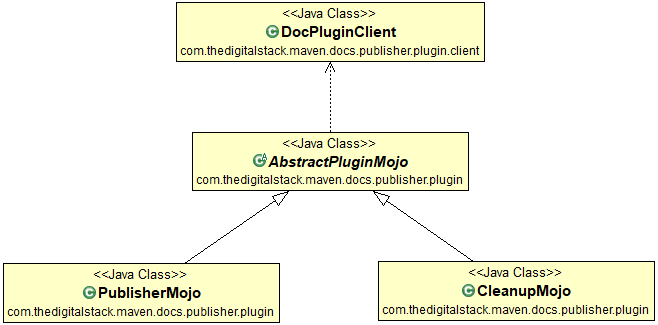
\includegraphics[width=0.8\textwidth]{immagini/PackageDiagram.png}\\
    \caption{Diagramma dei package}
\end{figure}
Le classi principali di \emph{Maven documentation publisher plug-in} sono i \emph{mojos} di Maven e il client.
Un \emph{mojo} è un \emph{goal} eseguibile in Maven, ovvero la classe che concretamente realizza lo scopo prefissato \cite{site:maven-mojo}. \\
I mojos appartengono al package Java \\ \texttt{com.thedigitalstack.maven.docs.publisher.plugin} e il client al sub-package\\ \texttt{com.thedigitalstack.maven.docs.publisher.plugin.client}.
Tra loro è possibile identificare due classi fondamentali: PublisherMojo e CleanupMojo.
Entrambe sono mojos di Maven e perciò rappresentano \emph{goal} differenti. \\
Alcuni metodi che riguardano il client e le impostazioni del server sono uguali, per questo motivo esiste una classe base e un riferimento a DocPluginClient.
DocPluginClient svolge le operazioni lato client ed è l'unico oggetto che comunica direttamente con Confluence.

\clearpage


%**************************************************************
\section{Diagrammi delle classi}
\label{sec:diagrammi-classi}

\subsection{Diagramma dei mojo} \label{diagrammiMojo}

\begin{figure}[H]
    \centering
    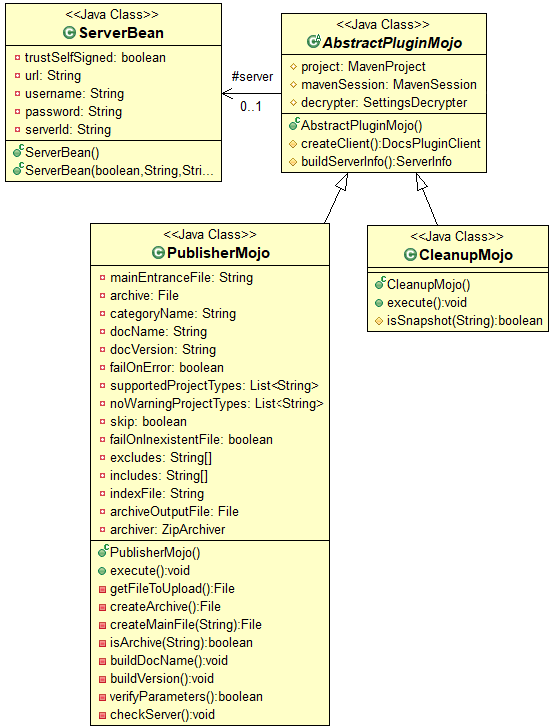
\includegraphics[width=0.85\textwidth]{immagini/mojo-gerarchy.png}\\
    \caption{Diagramma delle classi relativo alla gerarchia principale del plugin}
    \label{diagrammaMojo}
\end{figure}

\txt{PublisherMojo} realizza la pubblicazione della documentazione su Confluence, per questo motivo, il suo goal è nominato \emph{publish} e la fase del ciclo di vita Maven a cui è legato è \emph{package} di default. \\
Nella tabella \ref{tabellaParametri} è possibile vedere tutti i parametri configurabili dall'utente che, come è possibile notare, coincidono con i campi dati di PublisherMojo visibili nella figura \ref{diagrammaMojo}.
Ognuno di essi è seguito da una descrizione che li definisce e dal loro valore di default.

\begin{table}[H]
    \centering
    {\def\arraystretch{1.7}
    \begin{tabularx}{\textwidth}{cXX}
        \rowcolor{beautyblue} \textbf{Parametro} & \textbf{Descrizione} & \textbf{Valore di default} \\\toprule
        \txt{archive} & Documentazione da pubblicare & - \\
        \txt{server} & Java bean con le informazioni del server & \txt{trustSelfSigned}=false
        \txt{url}=https://jira-dev.fx.lan/confluence/
        \txt{serverId}=my.server \\
        \txt{categoryName}  & Nome della categoria scelta come posizione della documentazione & - \\
        \txt{docName} & Nome della documentazione & Nome del progetto, altrimenti l'artifactId del progetto \\
        \txt{docVersion} & Versione della documentazione & Versione del progetto \\
        \txt{failOnError} & Fallimento dell'esecuzione se si verifica qualche errore nel client & true \\
        \txt{supportedProjectTypes} & Lista dei tipi di progetto supportati dal plugin & jar, war, maven-plugin, eclipse-plugin \\
        \txt{noWarningProjectTypes} & Lista dei tipi di progetto a cui il plugin non deve sollevare warning se l'esecuzione viene saltata & pom \\
        \txt{ski}p & Salta l'esecuzione del plugin & false \\
        \txt{failOnInexistentFile} & Fallisce l'esecuzione del plugin se \txt{archive} non esiste, altrimenti salta l'esecuzione del plugin & true \\
        \txt{indexFile} & Nome del file HTML principale dell'archivio & index.html \\
        \txt{archiveOutputFile} & Percorso in cui salvare il nuovo archivio creato & \$\{project.build.directory\}/ docpublisher/archive.zip \\
        \txt{includes} & Lista dei file da includere nel nuovo archivio & **/** \\
        \txt{excludes} & Lista dei file da escludere dal nuovo archivio & **/*.git, **/*.svn, **/*.gitignore 
        \\\bottomrule
    \end{tabularx}}
    \caption{Parametri configurabili dall'utente}
    \label{tabellaParametri}
\end{table}

Come spiegato nella sezione \S\ref{goalPublish}, i primi tre parametri della tabella \ref{tabellaParametri} sono necessariamente richiesti all'utente per l'esecuzione del goal publish, mentre i successivi sono opzionalmente configurabili e per questo motivo, presentano tutti dei valori di default utilizzabili dal sistema qualora l'utente non li specificasse.

\txt{CleanupMojo} si occupa dell'eliminazione completa delle pagine \emph{doc} contenenti SNAPSHOT.
Ciò significa tutta la documentazione la cui versione comprende il qualificatore ``-SNAPSHOT''.
Per questo motivo, il goal relativo si chiama \emph{cleanup} e non è specificata nessuna fase del ciclo di vita di un progetto Maven.
Esso non richiede altri parametri in uso dall'utente: fa semplicemente affidamento sul metodo \txt{isSnapshot()} per comprendere se il titolo valutato è un ``-SNAPSHOT''.

PublisherMojo e CleanupMojo estendono \txt{AbrasctPluginMojo}.
Questa classe astratta estende \txt{AbrasctMojo} (la classe astratta base di qualunque mojo Maven) e definisce i metodi in comune ad entrambi, come per esempio \txt{createClient()} per l'inizializzazione del client, lasciando implementare il metodo \txt{execute()}, che permette l'esecuzione del goal, alle sottoclassi.

AbstractPluginMojo fa uso di un oggetto di tipo \txt{ServerBean}.
Un Java Bean è una classe utilizzata per incapsulare più oggetti in un oggetto singolo, cosicché tali oggetti possano essere passati come un singolo oggetto bean invece che come multipli oggetti individuali \cite{site:java-bean}.
ServerBean infatti contiene altri oggetti relativi alle informazioni richieste per connettersi al server Confluence, come per esempio la URL e le credenziali dell'utente.
Esso richiede inoltre il booleano \txt{trustSelfSigned} per determinare se i certificati SSL sono accettati, e una stringa \txt{serverId} nel caso l'utente volesse permettere di ricavare le credenziali dal file ``settings.xml''.

\subsection{Diagramma del client}

\begin{figure}[H]
    \centering
    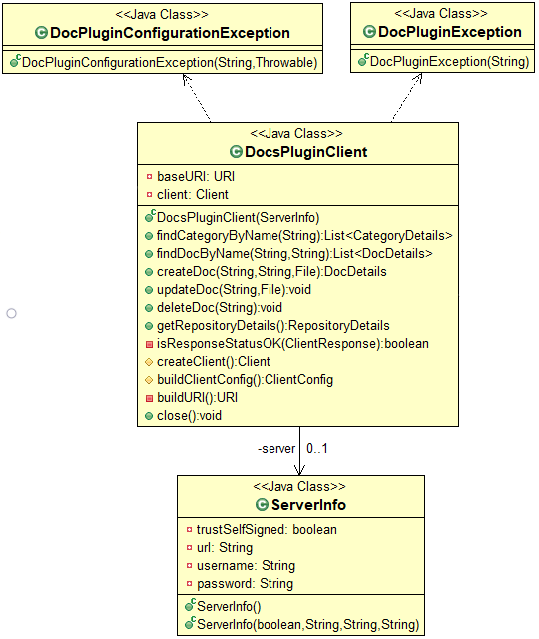
\includegraphics[width=0.83\textwidth]{immagini/client.png}\\
    \caption{Diagramma delle classi relativo al client}
\end{figure}

Il client è creato da AbstractPluginMojo ed è un oggetto di tipo \txt{DocsPluginClient}.
Questa classe fornisce tutto il necessario per creare ed usare un'istanza del client Jersey: riceve le informazioni per la configurazione da \txt{ServerInfo} (un semplice Java bean simile a ServerBean) e produce la directory di base richiesta per svolgere qualunque tipo di chiamata REST.

I metodi che compiono delle chiamate REST \cite{site:rest-docs} sono elencati nella tabella \ref{tabellaREST}.

\begin{table}[H]
    \begin{paddedtablex}[1.7]{\textwidth}{XcX}
        \rowcolor{beautyblue}\textbf{Nome} & \textbf{Richiesta} & \textbf{Descrizione} \\
        \toprule

        \txt{findCategoryByName(String categoryName)} & \bd{GET} & Ritorna una lista di categorie esistenti, il cui nome coincide con la stringa data \\
        \txt{findDocByName(String categoryId, String docName)} & \bd{GET}  & Ritorna una lista di doc esistenti all'interno di una categoria i cui nomi coincidono con la stringa data \\
        \txt{createDoc(String categoryId, String docName, File docArchive)} & \bd{PUT} & Crea la pagina doc all'interno di una categoria esistente, con l'archivio e il nome dato \\
        \txt{updateDoc(String docKey, File docArchive)} & \bd{POST} & Aggiorna la pagina doc identificata dalla \txt{docKey} data, con l'archivio dato \\
        \txt{getRepositoryDetails()} & \bd{GET} & Ritorna tutti i dettagli relativi alla repository: tutte le categorie e i doc esistenti \\
        \txt{deleteDoc(String docKey)} & \bd{DELETE} & Elimina la pagina doc relativa alla \txt{docKey} data \\

        \bottomrule
    \end{paddedtablex}
    \caption{Metodi di DocsPluginClient che compiono chiamate REST}
    \label{tabellaREST}
\end{table}

Molti di questi metodi possono tirare un'eccezione di tipo \txt{DocPluginException} quando il client riceve una risposta inaspettata da Confluence in fase di comunicazione.


Un'altra eccezione che DocsPluginClient può tirare è \txt{DocPluginConfigurationException}: un'eccezione RuntimeException che può avvenire durante la creazione del client.

\clearpage

\subsection{Diagramma delle componenti del plugin Docs}

\begin{figure}[H]
    \centering
    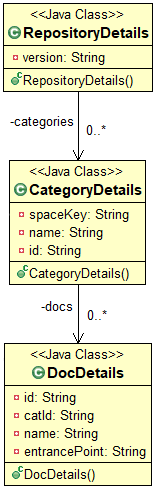
\includegraphics[width=0.24\textwidth]{immagini/details.png}\\
    \caption{Diagramma delle classi relativo ai dettagli di ogni componente del plugin Confluence}
\end{figure}

È importante specificare che una chiamata REST, come per esempio una di quelle di tipo GET, ottiene le specifiche di una categoria o un \emph{doc} tramite un file JSON.
Questi JSON sono trasformati da JAXB in oggetti Java.
A questo scopo, sono state create le seguenti classi:
\begin{itemize}
    \item \txt{RepositoryDetails}: informazioni sulla repository (comprende a sua volta tutte le informazioni sulle categorie e i loro \emph{doc});
    \item \txt{CategoryDetails}: informazioni sulla categoria (comprende a sua volta tutti i \emph{doc} contenuti);
    \item \txt{DocDetails}: informazioni sulla pagina \emph{doc}.
\end{itemize}

\clearpage

    \subsection{Riepilogo delle classi}

    \begin{table}[H]
		\begin{paddedtablex}[1.7]{\textwidth}{cX}
			\rowcolor{beautyblue}\textbf{Nome} & \textbf{Breve descrizione} \\
			\toprule

			\txt{AbstractPluginMojo} & Classe astratta dei mojos del plugin \\
            \txt{CleanupMojo} & Classe mojo coincidente con il \emph{goal cleanup}: elimina la documentazione ``SNAPSHOT'' \\
            \txt{PublisherMojo} & Classe mojo coincidente con il \emph{goal publish}: pubblica la documentazione software \\
            \txt{DocsPluginClient} & Client del plugin che realizza chiamate REST \\
            \txt{RepositoryDetails} & Oggetto Java che corrisponde al JSON riguardante i dettagli della repository \\
            \txt{CategoryDetails} & Oggetto Java che corrisponde al JSON riguardante i dettagli di una categoria \\
            \txt{DocDetails} & Oggetto Java che corrisponde al JSON riguardante i dettagli di un \emph{doc} \\
            \txt{ServerBean} & Java bean contenente le informazioni del sever \\
            \txt{DocsPluginException} & Eccezione sollevata da \txt{DocsPluginClient} per problemi durante la comunicazione con il server \\
            \txt{DocsPluginConfigurationException} & RunTimeException sollevata da \txt{DocsPluginClient} per problemi di configurazione \\

			\bottomrule
		\end{paddedtablex}
		\caption{Elenco delle classi}
	\end{table}


\clearpage


\section{Diagrammi di sequenza}
\label{sec:diagrammi-sequenza}

\subsection{Diagramma del goal \emph{publish}}
Ecco come funziona la pubblicazione della documentazione:

\begin{figure}[H]
    \centering
    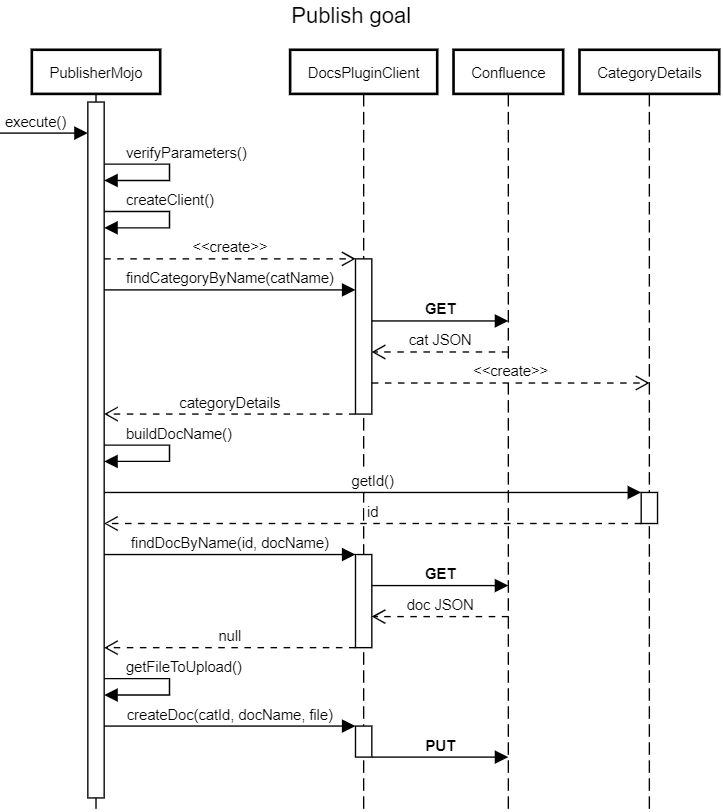
\includegraphics[width=\textwidth]{immagini/SeqPublish.png}\\
    % 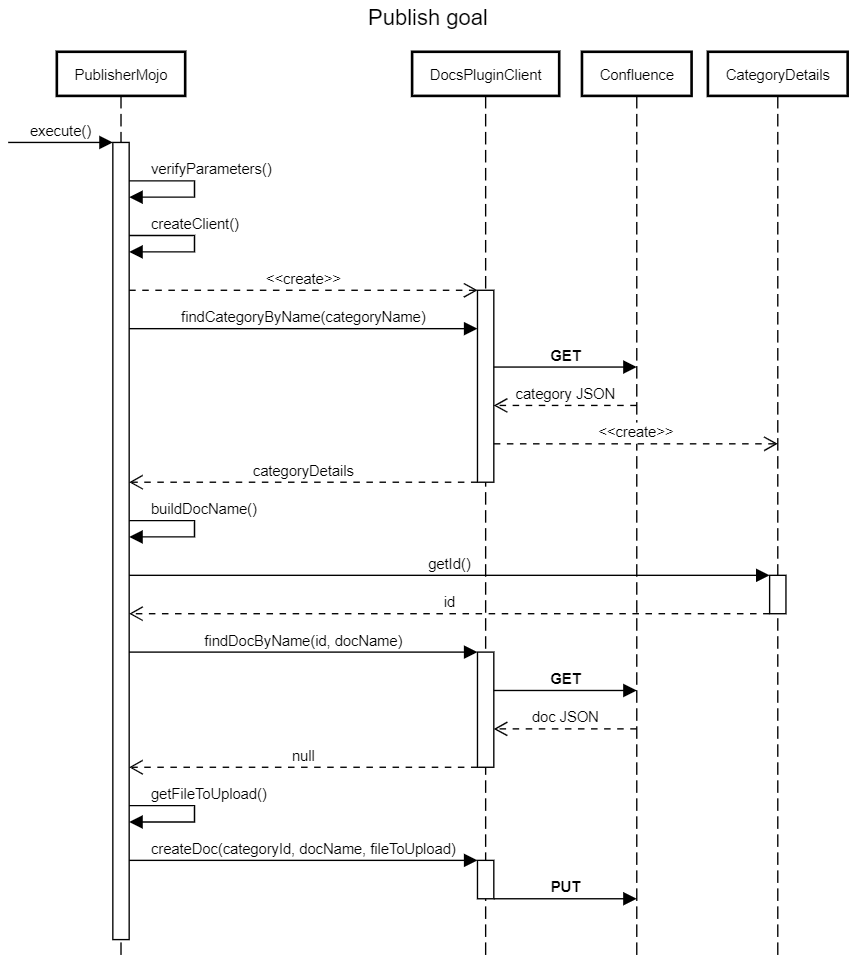
\includegraphics[width=\textwidth]{immagini/CreateDocSequence.png}\\
    \caption{Diagramma di sequenza relativo al \emph{goal publish}}
\end{figure}

Quando PublisherMojo viene eseguito, esso verifica la correttezza dei parametri dati e sospende l'esecuzione se necessario (per esempio se \txt{skip} è \txt{true}, ecc).

Dopo di che un'istanza di DocsPluginClient viene creata in modo da permettere le operazioni del client.
PublisherMojo usa DocsPluginClient per ricevere i dettagli della categoria appartenente al nome dato in fase di configurazione dall'utente.
Questo accade perché DocsPluginClient comunica con Confluence.
Il JSON che esso riceve da Confluence è trasformato nel relativo oggetto Java CategoryDetails.

Successivamente PublisherMojo costruisce il titolo della pagina \emph{doc} tramite nome e versione della documentazione.
In questo modo è possibile trovare il \emph{doc} con quel determinato titolo.
PublisherMojo ottiene l'id della categoria dall'oggetto precedentemente creato e richiede al client di trovare il \emph{doc} all'interno di quella categoria.

In questo caso, il JSON ritornato sarà vuoto perché la pagina \emph{doc} ancora non esiste.
A questo punto PublisherMojo ottiene l'archivio da pubblicare, che sarà l'archivio dato dall'utente o un nuovo archivio generato.

Infine la pagina \emph{doc} può essere creata all'interno della categoria con il nome e l'archivio selezionati. \\


L'aggiornamento di una pagina \emph{doc} funziona in maniera molto similare.
Le uniche differenze dallo scenario precedente si trovano dal JSON riguardante il \emph{doc} ritornato da Confluence in poi.
Esso non sarà vuoto, bensì conterrà le informazioni del \emph{doc} esistente.
A questo punto verrebbe chiamato un oggetto di tipo DocDeatails e il metodo \txt{udpateDoc()} verrebbe chiamato al posto di \txt{createDoc()}.


\subsection{Diagramma del goal \emph{cleanup}}

% \begin{figure}[H]
%     \centering
%     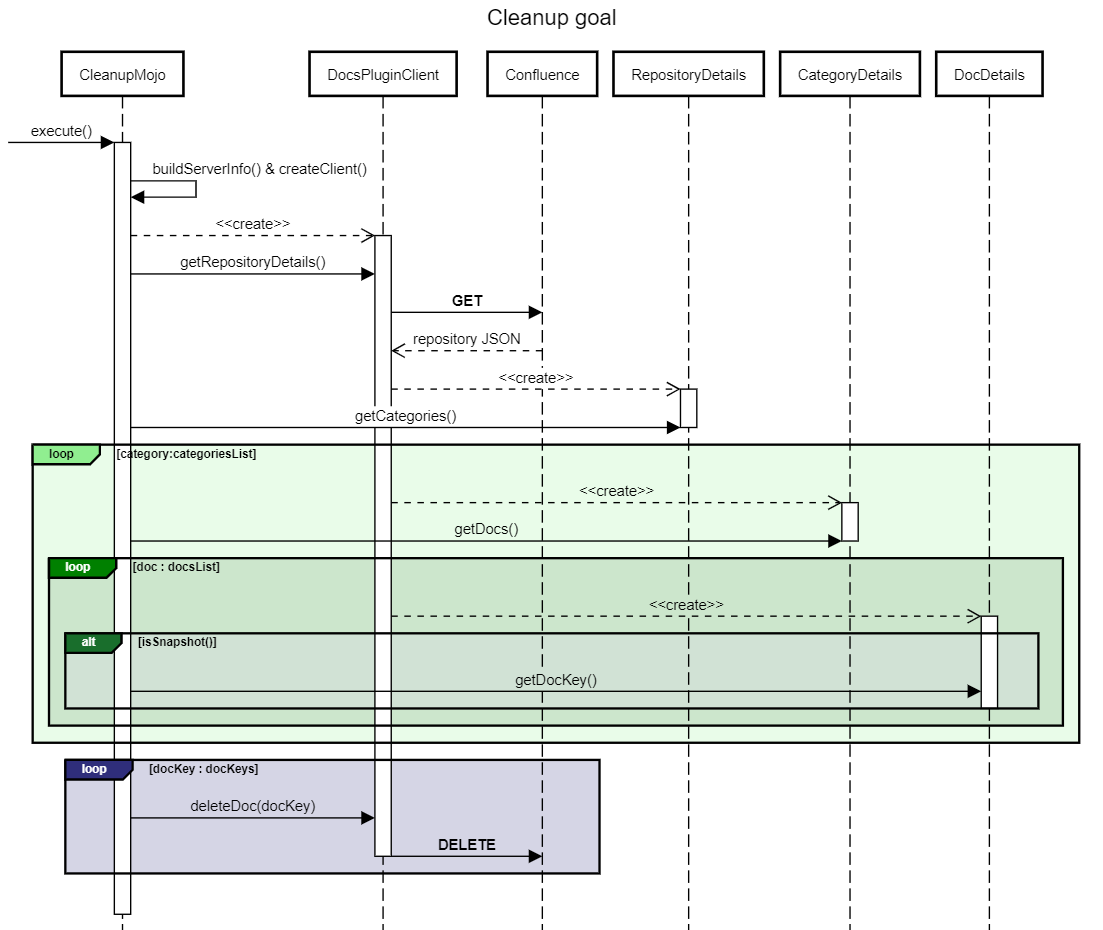
\includegraphics[width=\textwidth]{immagini/SequenceCleanupConfluence.png}\\
%     \caption{Diagramma di sequenza relativo al \emph{goal cleanup}}
% \end{figure}

\begin{figure}[H]
    \centering
    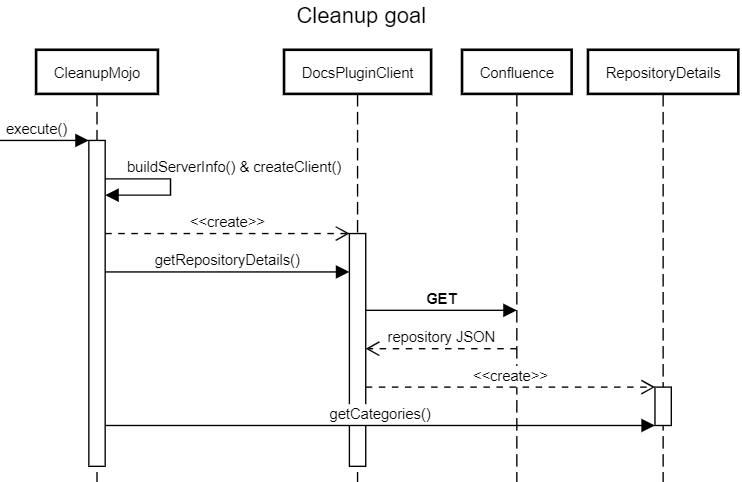
\includegraphics[width=\textwidth]{immagini/CleanupSeq1.png}\\
    \caption{Diagramma di sequenza relativo al \emph{goal cleanup} (1)}
\end{figure}

Prima di tutto, CleanupMojo agisce come PublisherMojo: crea un DocsPluginClient.
Grazie ad esso ottiene i dettagli relativi alla repository attraverso una chiamata GET a Confluence.
Il JSON ricevuto come risposta viene trasformato in un oggetto Java RepositoryDetails.
CleanupMojo ricava la lista di categorie dal RepositoryDetails precedentemente creato e itera su di esso.

\begin{figure}[H]
    \centering
    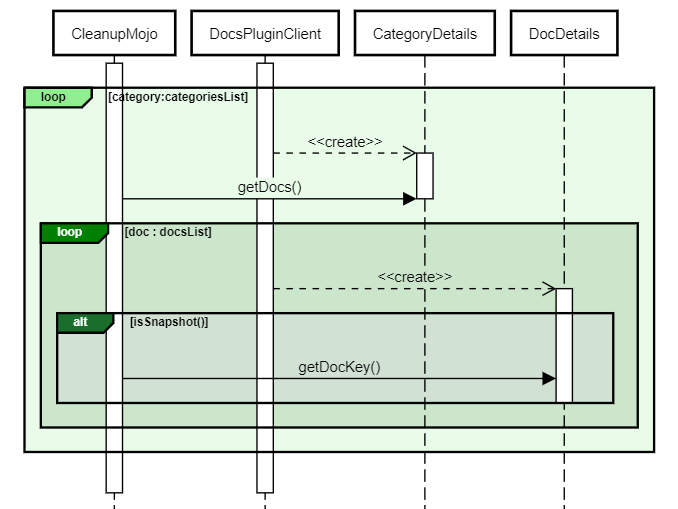
\includegraphics[width=\textwidth]{immagini/CleanupSeq2.png}\\
    \caption{Diagramma di sequenza relativo al \emph{goal cleanup} (2)}
\end{figure}

A questo punto richiede ad ogni CategoryDetails la sua lista di \emph{doc}.
Itera su ogni \emph{doc} controllandone il titolo per verificare se contiene ``SNAPSHOT''.
Se questa condizione è verificata, viene presa la chiave identificativa del \emph{doc} (\txt{docKey}).

\begin{figure}[H]
    \centering
    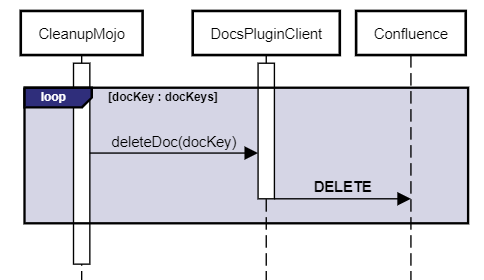
\includegraphics[width=0.75\textwidth]{immagini/CleanupSeq3.png}\\
    \caption{Diagramma di sequenza relativo al \emph{goal cleanup} (3)}
\end{figure}

Infine CleanupMojo elimina ogni pagina \emph{doc} all'interno del plugin Confluence \emph{Docs} di cui possiede l'identificativo.



\section{Configurazione} \label{configurazioneSec}
\lstset{frame=tb,
  language=Java,
  aboveskip=3mm,
  belowskip=3mm,
  showstringspaces=false,
  columns=flexible,
  basicstyle={\small\ttfamily},
  numbers=none,
  numberstyle=\tiny\color{black},
  keywordstyle=\color{black},
  commentstyle=\color{black},
  stringstyle=\color{black},
  breaklines=true,
  breakatwhitespace=true,
  tabsize=3
}
La configurazione è una parte predominante di Maven documentation publisher plug-in, poiché è l'unico momento un cui l'utente ha potere di decisione.
Come già precedentemente spiegato nella sezione \S\ref{mavenSection}, tutte le informazioni di configurazione del progetto risiedono nel file ``pom.xml'' \cite{site:maven-plugin-configurazione}.
Per questo motivo, bisogna innanzitutto aggiungere il plugin al proprio progetto inserendo le informazioni che lo identificano:

\begin{lstlisting} 
<project>
    ...
    <build>
        ...
        <plugins>
            <plugin>
                <groupId>com.thedigitalstack.maven.plugins</groupId>
                <artifactId>tds-docs-publisher-plugin</artifactId>
                <version>1.3.1-SNAPSHOT</version>
            </plugin>
        </plugins>
    <build>
</project>
\end{lstlisting}

Dopo di che, la configurazione ideale per il plugin varia in base alla preferenza dell'utente.\footnote{Tutti gli elementi mostrati negli esempi a seguire, sono i parametri della tabella \ref{tabellaParametri} presente nella sezione \S\ref{diagrammiMojo}.}
Se il goal che si vuole eseguire è \emph{cleanup}, è sufficiente aggiungere le informazioni del server con le proprie credenziali.

\begin{lstlisting}
<plugin>
    <groupId>com.thedigitalstack.maven.plugins</groupId>
    <artifactId>tds-docs-publisher-plugin</artifactId>
    <version>1.3.1-SNAPSHOT</version>
    <configuration>
        <server>
            <trustSelfSigned>false</trustSelfSigned>
            <url>https://jira-dev.fx.lan/confluence/</url>
            <username>${env.USERNAME}</username>
            <password>${env.PASSWORD}</password>
            <serverId>my.server</serverId>
        </server>
    </configuration>
</plugin>
\end{lstlisting}

Nell'esempio sopra, sono stati dati entrambi i modi per ottenere le credenziali dell'utente: sia tramite \txt{serverId} che tramite username e password grazie a delle variabili d'ambiente.

Se il goal che si vuole eseguire è invece \emph{publish}, la configurazione richiede anche l'archivio della documentazione da pubblicare e il nome della categoria.

\clearpage

\begin{lstlisting}
<plugin>
    <groupId>com.thedigitalstack.maven.plugins</groupId>
    <artifactId>tds-docs-publisher-plugin</artifactId>
    <version>1.3.1-SNAPSHOT</version>
    <configuration>
        <server>
            <trustSelfSigned>false</trustSelfSigned>
            <url>https://jira-dev.fx.lan/confluence/</url>
            <username>${env.USERNAME}</username>
            <password>${env.PASSWORD}</password>
            <serverId>my.server</serverId>
        </server>
        <archive>${project.basedir}/target/${project.artifactId}-
        ${project.version}-javadoc.jar</archive>
        <categoryName>Category</categoryName>
    </configuration>
</plugin>
\end{lstlisting}

La configurazione sopra mostrata va bene solo nel caso il cui la documentazione sia già un archivio (come in questo caso, un JAR) o un file HTML (in quel caso l'elemento \txt{archive} conterrebbe il percorso ad il file HTML).

Nel caso in cui la documentazione fosse una cartella, è necessaria l'archiviazione, quindi la configurazione (scegliendo di tenere i valori di default dei parametri) sarebbe per esempio:

\begin{lstlisting}
<configuration>
    <server>
        <trustSelfSigned>false</trustSelfSigned>
        <url>https://jira-dev.fx.lan/confluence/</url>
        <username>${env.USERNAME}</username>
        <password>${env.PASSWORD}</password>
        <serverId>my.server</serverId>
    </server>
    <categoryName>Category</categoryName>
    <archive>C:\Path\...\doc</archive>
    <archiveOutputFile>${project.build.directory}/docpublisher/
    archive.zip</archiveOutputFile>   
    <includes>   
        <include>**/**</include>
    </includes>
    <excludes>
        <exclude>**/*.git</exclude>
        <exclude>**/*.svn</exclude>
        <exclude>**/*.gitignore</exclude>
    </excludes>
</configuration>
\end{lstlisting}

Questo perché l'archivio verrà salvato nel percorso e col nome specificato da \txt{archiveOutputFile}.
Inoltre, gli elementi \txt{includes} e \txt{excludes} definiscono i file della cartella da inserire o meno nel nuovo archivio.

Nel caso in cui la documentazione data non contenesse il file ``index.html'', la \emph{main entrance page} richiesta dal plugin Docs di Confluence, la configurazione sarebbe uguale alla precedente, con l'aggiunta dell'elemento \txt{indexFile}.
Questo elemento richiede come valore il nome del file che l'utente sceglie come file principale della documentazione data, ad esempio \txt{<indexFile>home.html</indexFile>}.\\


La configurazione per il titolo della pagina doc avviene tramite i parametri \txt{docName} e \txt{docVersion}, come:
\begin{lstlisting}
<configuration>
    ...
    <docName>Docs Maven Plugin</docName>
    <docVersion>2019</docVersion>
</configuration>
\end{lstlisting}
per ottenere il titolo ``Docs Maven Plugin 2019''.

Per quel che riguarda gli altri parametri del plugin inerenti allo skip dell'esecuzione, la configurazione (seguendo sempre i valori di default) sarebbe:

\begin{lstlisting}
<configuration>
    ...
    <failOnError>true</failOnError>
    <skip>false</skip>
    <supportedProjectTypes>
        <supportedProjectType>jar</supportedProjectType>
        <supportedProjectType>war</supportedProjectType>
        <supportedProjectType>maven-plugin</supportedProjectType>
        <supportedProjectType>eclipse-plugin</supportedProjectType>
    </supportedProjectTypes>
    <noWarningProjectTypes> 
        <noWarningProjectType>pom</noWarningProjectType>
    </noWarningProjectTypes>
    <failOnInexistentFile>true</failOnInexistentFile>
</configuration>
\end{lstlisting}

    \subsection{Proprietà}
    Ognuno di questi elementi configurabili può essere personalizzato dall'utente anche tramite l'utilizzo delle proprietà.
    Una proprietà è composta da \txt{tds.docpublisher.} e il nome dell'elemento. Essa va aggiunta all'elemento \txt{properties} del POM, come ad esempio:
        \begin{lstlisting}
        <project>
            ...
            <properties>
                <tds.docpublisher.skip>true</tds.docpublisher.skip>
            </properties>
            ...    
        </project>
        \end{lstlisting}

\clearpage

\section{Esecuzione}    \label{secEsecuzione}
Per eseguire il goal \emph{publish} può essere lanciato sul progetto Maven qualunque comando che comprenda la fase di \emph{package}, come per esempio:
\begin{lstlisting} 
    mvn install
\end{lstlisting}
Questo perché \emph{install} è la fase del ciclo di vita del progetto in cui Maven installa il pacchetto (JAR) nella repository locale, per poterlo usare come dipendenza in altri progetti locali \cite{site:maven-lifecycle}.
Lanciando questo comando quindi, vengono eseguite anche tutte la fasi precedenti.\\

Per il goal \emph{cleanup} invece, non essendo legato a nessuna fase, è necessario invocare esplicitamente il goal del plugin, ovvero lanciare:
\begin{lstlisting} 
    mvn tds-docs-publisher-plugin:cleanup
\end{lstlisting}

% \clearpage

\section{Documentazione}    \label{secDocumentazione}
Oltre al plugin Maven, altri due prodotti sono stati realizzati per questo progetto: il manuale utente e il manuale dello sviluppatore.

    \subsection{Manuale utente}
    Il manuale dell'utilizzatore ha il compito di descrivere le possibili configurazioni del plugin per semplificarne l'utilizzo allo sviluppatore.
    Esso è suddiviso in due artefatti:
    \begin{itemize}
        \item una pagina di documentazione Confluence;
        \item una pagina di utilizzo Maven \emph{Usage}.
    \end{itemize}
    Entrambe hanno essenzialmente lo stesso contenuto, ma la pagina Confluence è simile ad un documento Word con testo e immagini, mentre la pagina Maven di Usage presenta una struttura diversa.

        \subsubsection{Usage}
        Per realizzare una pagina di Usage è necessario comprendere la sintassi del linguaggio APT.
        APT sta per ``Almost Plain Text'' ed è un linguaggio di markup che è stato creato con l'obiettivo di semplificare la scrittura e la struttura della documentazione Maven \cite{site:apt}.
        La sua sintassi assomiglia al plain-text (testo non formattato) e permette la generazione automatica di una pagina web, come mostrato dalle prossime immagini.

        Il pezzo di file APT mostrato in figura \ref{usageAPT} \cite{site:apt-file}, correttamente eseguito durante il ciclo di vita Maven denominato \emph{site}, crea la parte di pagina HTML di Usage della figura \ref{usageImage} \cite{site:maven-usage}.

        \begin{figure}[H]
            \centering
            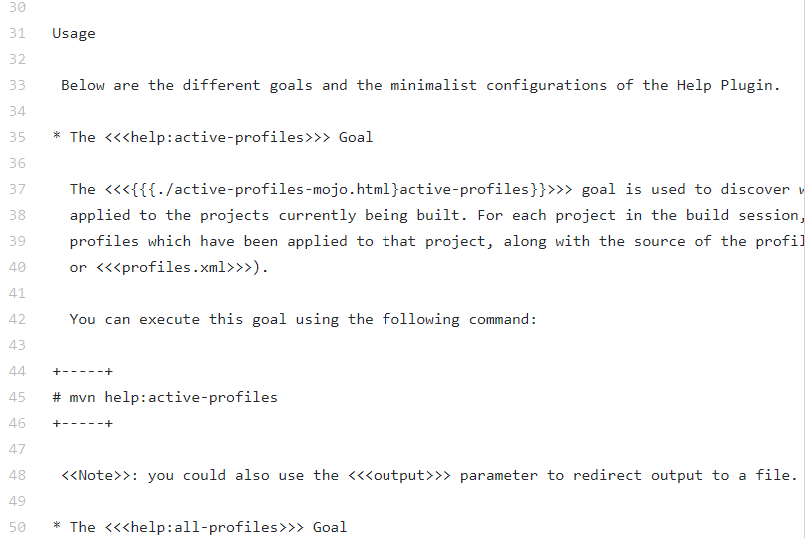
\includegraphics[width=0.9\textwidth]{usageAPT}\\
            \caption{Esempio di un file in formato APT}
            \label{usageAPT}
        \end{figure}

        \begin{figure}[H]
            \centering
            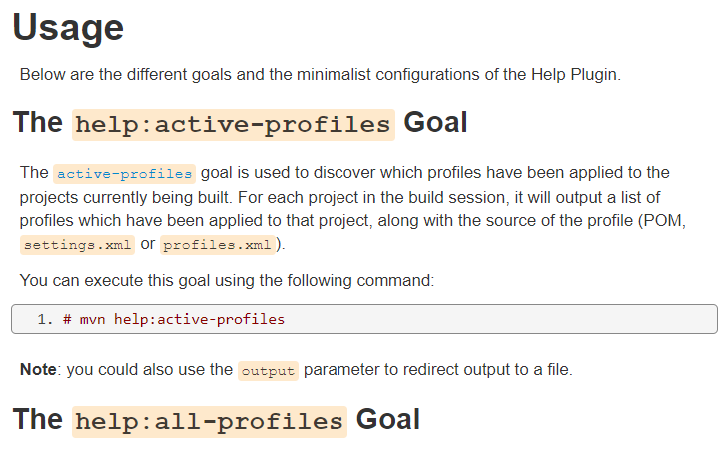
\includegraphics[width=0.9\textwidth]{usagePage}\\
            \caption{Esempio di pagina di Usage Maven}
            \label{usageImage}
        \end{figure}

        La pagina di Usage realizzata per questo progetto è simile all'esempio sopra riportato: spiega i due goal del plugin, \emph{publish} e \emph{cleanup}, con le stesse informazioni presenti in questo documento alla sezione \S\ref{descrizioneProdotto}, e con le istruzioni per la configurazione e l'esecuzione come esposti nelle sezioni \S\ref{configurazioneSec} e \S\ref{secEsecuzione}.

    \subsection{Manuale sviluppatore}
    Il manuale del programmatore garantisce una spiegazione dettagliata delle classi create per la realizzazione del plugin Maven.
    Anch'esso ha richiesto la creazione di due artefatti tecnici:
    \begin{itemize}
        \item una pagina di documentazione Confluence;
        \item documentazione JavaDoc.
    \end{itemize}
    La pagina Confluence comprende la descrizione di tutte le classi con il supporto di diagrammi dei package, delle classi e di sequenza, come le sezioni \S\ref{sec:diagramma-package}, \S\ref{sec:diagrammi-classi} e \S\ref{sec:diagrammi-sequenza} di questo documento.
    La specifica JavaDoc consta di tutti i dettagli rilevanti di ogni frammento di codice (metodi e campi dati), con i classici tag \cite{site:javadoc} quali per esempio:
    \begin{itemize}
        \item \txt{@author}: per inserire il nome dello sviluppatore;
        \item \txt{@param}: per definire i parametri di un metodo;
        \item \txt{@return}: per indicare il valore di ritorno di un metodo;
        \item \txt{@exception}: per indicare l'eccezione che il metodo può lanciare.
    \end{itemize}
    Sono state inoltre utilizzare le annotazioni di \txt{Nonnull} per segnalare campi che non posso avere valore nullo e \txt{Nullable} per indicare invece quali possono averlo.


%**************************************************************
% \section{Ciclo di vita del software}
% \label{sec:ciclo-vita-software}


%**************************************************************
% \section{Design Pattern utilizzati}

% \subsection{Template Method}

%**************************************************************
% \section{Codifica}
